
\section{Installing UIMA SDK}

Similar to the installation processes you have gone through for Git and Maven,
you will install the UIMA binaries and a UIMA Eclipse plug-in. Different from
the installation instruction you have learned from class or the official
tutorial, you \textbf{DO NOT} need to download the UIMA SDK, uncompress and copy
the archive into the Eclipse installation path. In fact, UIMA SDK will be
handled by the Maven archetype \verb|hw1-archetype| that we built for you for
this task, and the Eclipse plug-in for UIMA can be installed with the Eclipse
\textbf{Install New Software} function, which is basically the same as described
in the official tutorial, plus one tiny additional action you have to perform to
solve the dependency problem during installation.

\begin{enumerate}

\item As mentioned in the class and the official UIMA tutorial, you should
install Eclipse EMF plug-in, but if you strictly followed the instruction from
last homework, then EMF should have been installed as it is a default component
of Eclipse Juno for Java Developers. Otherwise, you should install it by
yourself.

\item Follow the instruction in subsection
3.1.2\footnote{\url{https://uima.apache.org/d/uimaj-2.4.0/overview_and_setup.html\#ugr.ovv.eclipse_setup.install_uima_eclipse_plugins}}
of the \emph{Overview \& Setup} section of \emph{UIMA Manuals and Guides} by
adding the UIMA Eclipse Plug-in Update site
(\url{http://www.apache.org/dist/uima/eclipse-update-site})

\item But, you might encounter a ``Cannot satisfy dependency'' issue like shown
in Figure \ref{fig:uima-01-dependency}. You can apply a workaround for this
year-long bug\footnote{You can find people asking about this issue since over a
year ago at
\url{http://www.mail-archive.com/user@uima.apache.org/msg00781.html}} by only
selecting the ``Apache UIMA Eclipse tooling and runtime support'' and
unselecting the ``Apache UIMA-AS (Asynchronous Scaleout) Eclipse tooling'' (as
shown in Figure \ref{fig:uima-02-tools}), where the latter tool will not be used
for this course.

\begin{figure}[t]
\centering
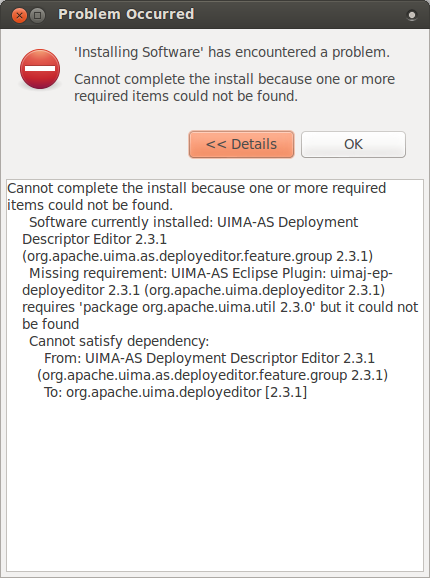
\includegraphics[scale=0.3]{uima-01-dependency}
\caption{Showing a ``Cannot satisfy dependency'' error\label{fig:uima-01-dependency}}
\end{figure}

\begin{figure}[t]
\centering
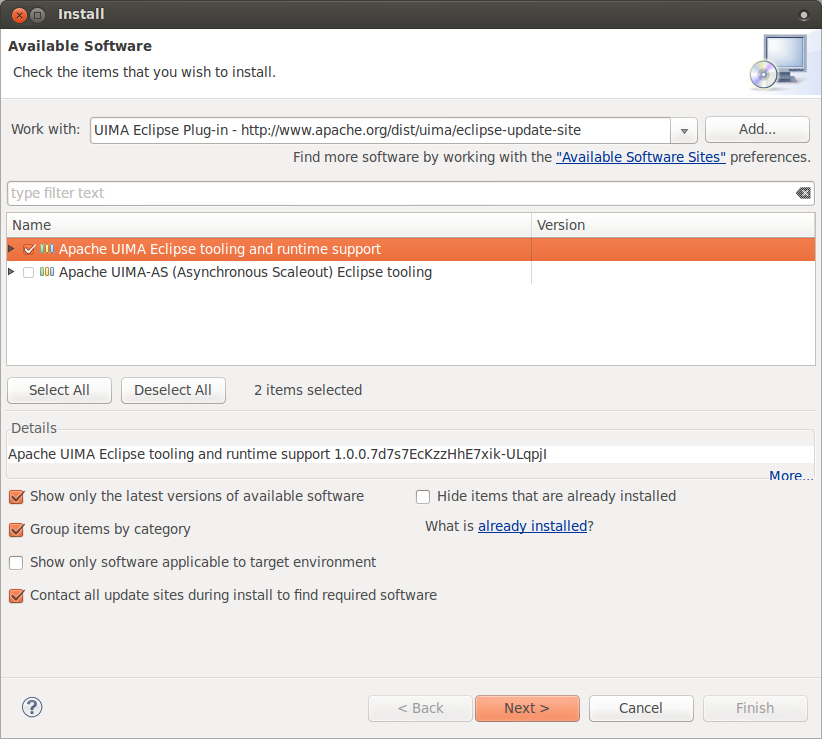
\includegraphics[scale=0.3]{uima-02-tools}
\caption{Using a workaround to solve the dependency error\label{fig:uima-02-tools}}
\end{figure}

\item After installation, you are able to create or edit UIMA descriptors with a
nice GUI.
 
\end{enumerate}
